\documentclass{mcmthesis}
\mcmsetup{CTeX = false,   % 使用 CTeX 套装时,设置为 true
        tcn = 55869, problem =  C,
        sheet = true, titleinsheet = true, keywordsinsheet = true,
        titlepage = false, abstract = true}
\problem{C}

\makeatletter % `@' now normal "letter"   %follpw as section test
\@addtoreset{equation}{section}
\makeatother  % `@' is restored as "non-letter"
\renewcommand\theequation{\oldstylenums{\thesection}%
                   .\oldstylenums{\arabic{equation}}}
\newcommand{\upcite}[1]{\textsuperscript{\textsuperscript{\cite{#1}}}}
\usepackage{palatino}
\usepackage{mwe}
\usepackage{graphicx}
\usepackage{tabularx}
\usepackage{float}
\usepackage{indentfirst}
\usepackage{amsmath}
\usepackage{caption}
\usepackage{subfigure}
\title{}
\date{}

\begin{document}

\begin{abstract}%摘要


\title{Keep the Bathtub Warm}



\end{abstract}

\begin{keywords}
	\textbf{A,\indent B, \indent}
\end{keywords}
\maketitle
\tableofcontents\thispagestyle{empty}
%设置页眉
\newpage

\setcounter{page}{1}
%Section 1
\section{Introduction}
\subsection{Literature review}
\indent Traffic flow modeling as the basis of traffic control, traffic design, traffic analysis, traffic simulation and traffic control decision making always is the the research focus in traffic engineering field. And it can be divided into macroscopic and microscopic models from the angle of study, mainly using the theory of fluid mechanics and the theory of car following. Due to their accuracy and practicability, these two models play an important role in the development of traffic flow modeling.\\
\indent The cellular automata (CA) is a kind of grid dynamical model in which time, space and state are discrete, and the space interaction and time causality are local. It has the ability to simulate the spatio-temporal evolution process of complex systems. The study of single lane traffic flow cellular automaton model began in 1986, the most famous of them is the NS model proposed by Nagel and Schreeckenberg in 1992$^{[2]}$. However, this model has a great flaw, and has been gradually improved by follow-up scientists. Such as the T2 model$^{[3]}$ put forward by Takayasu and the VDR model$^{[4]}$ put forward by barlovic. Cellular automata is now always used to calculate traffic flow problems.\\


\section{Assumptions}
\noindent
{\bf (1) } \textbf{example.} example.\\

\section{Symbols}
\begin{table}[H]
        \setlength{\abovecaptionskip}{0pt}
        \setlength{\belowcaptionskip}{0pt}
				\centering{Table 1:Constants}\\
        \begin{tabular}{p{2cm}|p{2cm}|p{7.5cm}|p{1.7cm}}
		\hline
		\rowcolor[gray]{0.9}\bf{Symbol}	&\bf{uint}      &\bf{Meaning}&\bf{value}	\\
		\hline
		${P}''_{v}$		& $hP_{a}$		 & example  &12\\

		\hline
		\end{tabular}
	\end{table}

\begin{table}[H]
        \setlength{\abovecaptionskip}{0pt}
        \setlength{\belowcaptionskip}{0pt}
        \centering{Table 2:Notation} \\
        \begin{tabular}{p{1.8cm}|p{2.2cm}|p{9cm}}
        \hline
        \rowcolor[gray]{0.9}\bf{Symbol}	&\bf{uint}      &\bf{Meaning}\\
        \hline
        $V(h)$			& $m^3  $		 & example \\
        \end{tabular}
        \end{table}

\section{Models}

\begin{equation}
\begin{split}
h=H(v)  \\
S_{1}=S_{1}(h) \\
S_{2}=S_{2}(h)  \\
\end{split}
\end{equation}
\indent example\\
\begin{itemize}
\item{Liquid surface heat loss model.\\ }
\item{contact area of liquid and bathtub heat loss model.\\ }
\end{itemize}
\subsection{The Set of Time Headway}
\indent Time Headway (TH) is the time difference between the two adjacent vehicles passing through the same location. In general, the TH is a random value. But when people drive a car, the front car has an emergency brake or deceleration in a very short time, the following car driver can respond only after a certain reaction time. It is easy to cause traffic accidents if the distance between the two cars is two small. So the HT between the two cars needs to be greater than a minimum safety HT. The safety HT is depended on the reaction time of person.\\
\indent The HT of two vehicles is determined by the subjective judgment of the driver. But generally speaking, when the rear car is far away from the front car, the rear car will speed up and make the HT of two cars smaller. When the driver of rear is aware that the HT is too small, as the HT of reality is less than the HT he expected, the driver will slow down and increase the HT between two cars.\\

\subsection{example}%TEST
 
\begin{figure}[H]
\centering
\subfigure[When Kp is too small]{
\begin{minipage}{7cm}
\centering 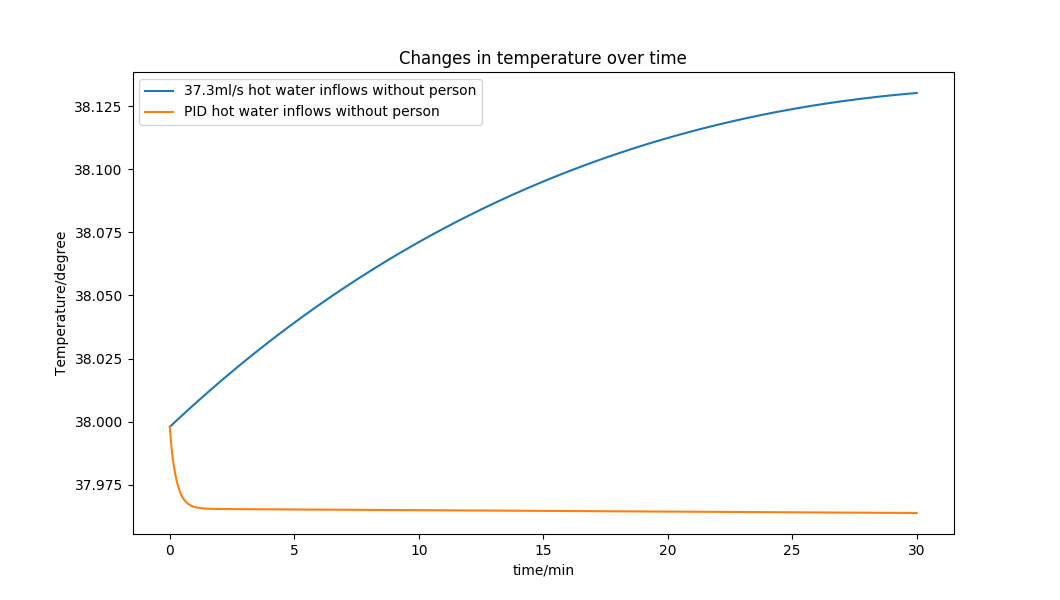
\includegraphics[scale=0.26]{PID_1.png}       
\end{minipage}
}
\subfigure[When Kp is too large]{
\begin{minipage}{7cm}
\centering                                    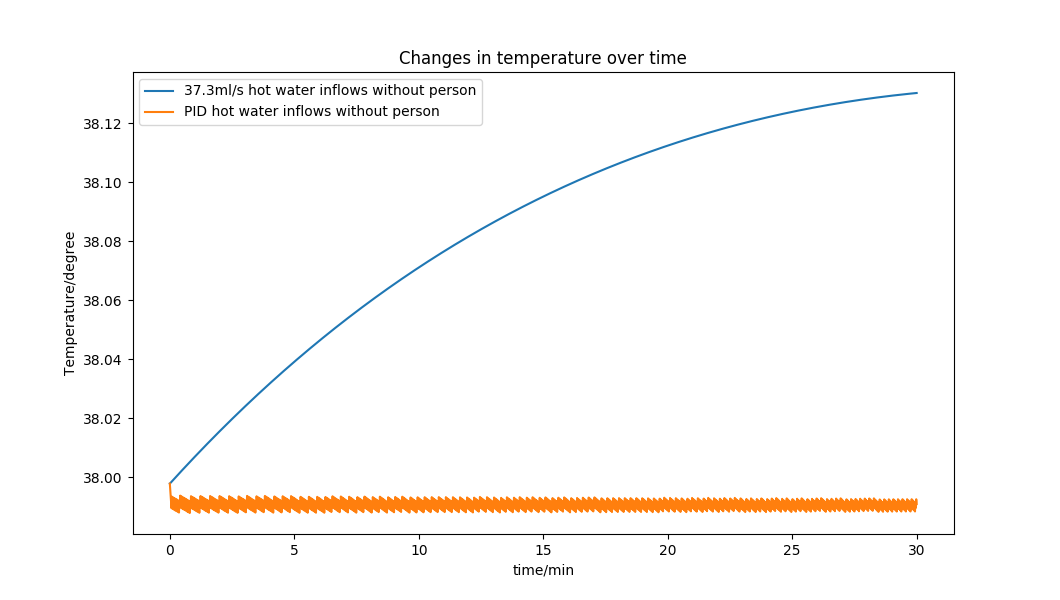
\includegraphics[scale=0.26]{PID_4.png}        
\end{minipage}
}
\caption{Only use Kp\upcite{test}}
\label{PID1}
\end{figure}


\section{Simulation Result and Data Analysis}

\section{Model Validation}

\section{Sensitivity Analysis}

\section{Strengths and Weaknesses}



\section{References}
\begin{thebibliography}{99}
\bibitem{test}Zhenguo Zhao. Formula of enthalpy difference for water surface heat dissipation and its application[J]. Journal of Hydraulic Engineering, 2004(02):34-38.

\end{thebibliography}



\end{document}